\section{Circular motion}
\subsection{Uniform circular motion}
\vocab{Uniform circular motion} is a type of motion in which an object moves at a \textit{constant speed} in a circular path.

\begin{defn}{Radian}{}
Unit of angular measure, defined as the angle subtended at the centre of a circle by an arc of a length equal to the radius of the circle.
\end{defn}

\vocab{Angular displacement} $\theta$ refers to the angle in radians through which a point is rotated.
\begin{equation} \theta = \frac{s}{r} \end{equation}

\begin{figure}[H]
    \centering
    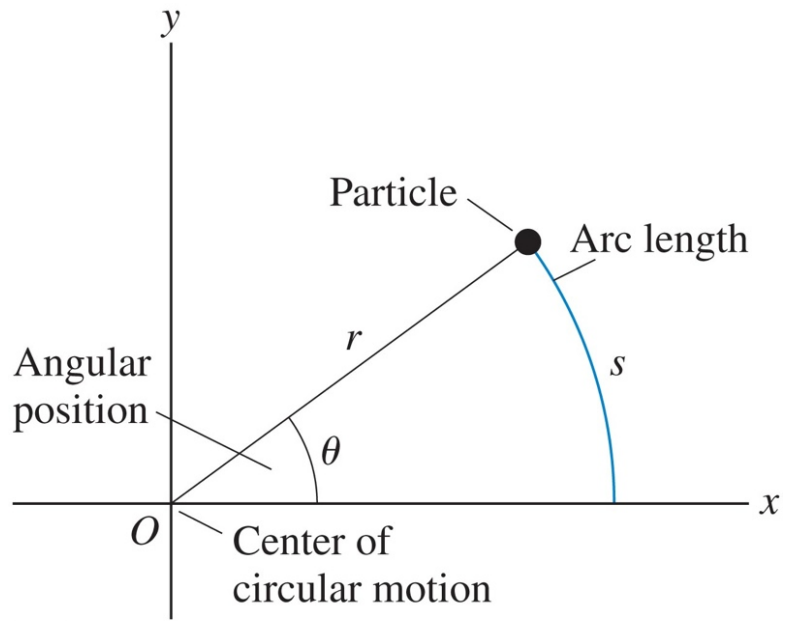
\includegraphics[width=8cm]{images/Angular_displacement.png}
\end{figure}

\vocab{Angular velocity} $\omega$ refers to rate of change of angular displacement.
\begin{equation} \omega = \dv{\theta}{t} \end{equation}

Relating angular velocity to period $T$ and frequency $f$, 
\begin{equation} \omega = \frac{2\pi}{T} = 2\pi f \end{equation}

\vocab{Linear velocity} $v$ is given by 
\begin{equation} v = r\omega \end{equation}

\vocab{Centripetal acceleration} $a$ is given by
\begin{equation} a = \frac{v^2}{r} = r\omega^2 \end{equation}

\vocab{Centripetal force} $F_c$ is given by
\begin{equation} F_c = \frac{mv^2}{r} = mr\omega^2 \end{equation}
\begin{remark}
Centripetal force is a \textbf{resultant force}; it can be provided by gravitational force, friction force, normal force, etc. 
\end{remark}

\begin{tcolorbox}
\textbf{Why does a resultant force exist in a uniform circular motion?}

Velocity changes due to change in direction, hence the object undergoes acceleration. By Newton's 2nd Law, a resultant force acts on the object. 

Since the force does not change the speed of the object, it does no work to accelerate the object, thus centripetal force acts \underline{perpendicularly} to motion, towards the \underline{centre} of the circle.
\end{tcolorbox}

\subsection{Non-uniform circular motion}
Consider an object rotating vertically in a circle of radius $r$.
\begin{figure}[H]
	\centering
	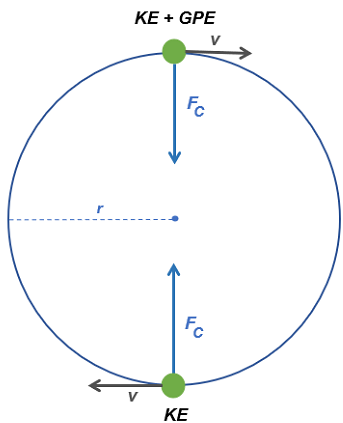
\includegraphics[width=6cm]{Vertical_circular_motion}
\end{figure}

Tension in the spring reaches maximum at the bottom and minimum at the top.

At the top, if the string is just taut, $mg$ provides centripetal force completely, $T=0\:\unit{N}$.
\begin{align*}
mg &= \frac{m{v_{\text{top}}}^2}{r}\\
v_{\text{top}} &= \sqrt{gr}
\end{align*}
At the bottom, by conservation of mechanical energy,
\begin{align*}
\frac{1}{2} m{v_{\text{bottom}}}^2 &= mg(2r) + \frac{1}{2} m{v_{\text{top}}}^2\\
v_{\text{bottom}} &= \sqrt{5gr}
\end{align*}
\pagebreak

\subsection*{Problems}
2014 P1 Q11, Q12, 2015 P1 Q10, 2016 P1 Q13, 2019 P1 Q10, 
2013 P2 Q3 (pg 7(7)) 
\pagebreak